\documentclass[10pt]{article}
\usepackage[a4paper,margin=17mm]{geometry}
\usepackage{amsmath,amssymb,graphicx,booktabs,hyperref,xcolor}
\hypersetup{colorlinks=true,urlcolor=blue}
\setlength{\parindent}{0pt}\setlength{\parskip}{4pt}
\begin{document}
{\LARGE Six-section elliptic relation predicate}\par
17 November 2026. Fixed native controls; producer unsigned/unverified.

\textbf{Result.} The new Rust predicate agrees with the existing native group
law on all 600 registered candidate/target cases. It produces 60 normalized
null sections, rejects 360 coefficient mutations and 33 malformed/unsupported
or certificate controls, and reproduces four false positives in naive
encodings. It checks \emph{supplied} points; it discovers no factor-base root.

\begin{center}\begin{tabular}{@{}lll@{}}
\toprule
Native field & Recorded value & Scope\\\midrule
planned / attempted / matched &600 / 600 / 600& Fixed comparison decisions\\
positive sections &60& Rank5 and checked coefficient vector\\
coefficient mutations refused &360& Six changes per positive section\\
naive counterexamples &4& Two defects in each field\\
other refusals &33& Errors/rejections, not relation absence\\\bottomrule
\end{tabular}\end{center}

\textbf{Exact domain.} $E:y^2=x^3+Ax^2+x$, with $p=101,A=95$ or
$p=2^{255}-19,A=486662$ in the fixed controls. Actual subgroup order is
$N=2^{252}+27742317777372353535851937790883648493$, cofactor8.
Native v1 admits only these fields, canonical nonsingular $A$, six finite
members with $y\ne0$ and distinct raw IDs, and target $O$ or finite $y\ne0$.
Geometric aliases are allowed. Identity members and finite2-torsion are
explicit unsupported errors, not negative decisions. Original membership,
index/sign decoding and cofactor provenance remain separate obligations.

\textbf{Construction.} For $R=(r,s)$, $s\ne0$, a basis of $L(5O+R)$ is
\[
 1,\;x,\;y,\;x^2,\;xy,\;h_R=\frac{y+s}{x-r}.
\]
For $R=O$ use $1,x,y,x^2,xy,x^3$ in $L(6O)$. Evaluate local sections and
all multiplicity jets to obtain a $6\times6$ matrix. Its kernel is
$L(5O+R-Z)$ for the degree-six effective multiset $Z$. The classical divisor
argument identifies singularity with $\sum_i P_i=R$. This is established
elliptic-code theory, not a new geometric theorem.

\begin{center}
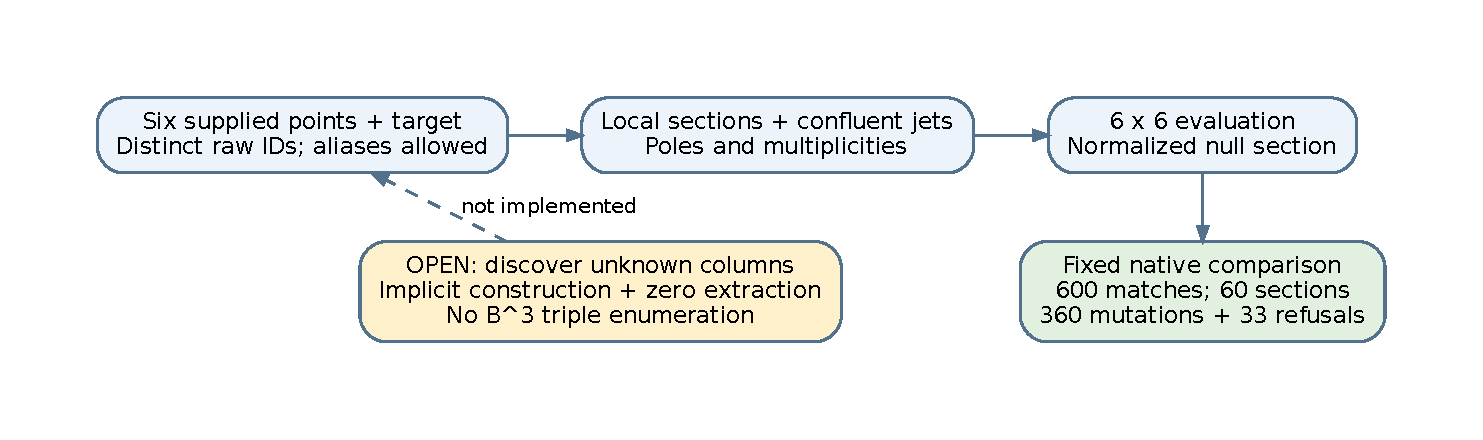
\includegraphics[width=\linewidth,height=37mm,keepaspectratio]{pipeline.pdf}
\end{center}
\begin{center}
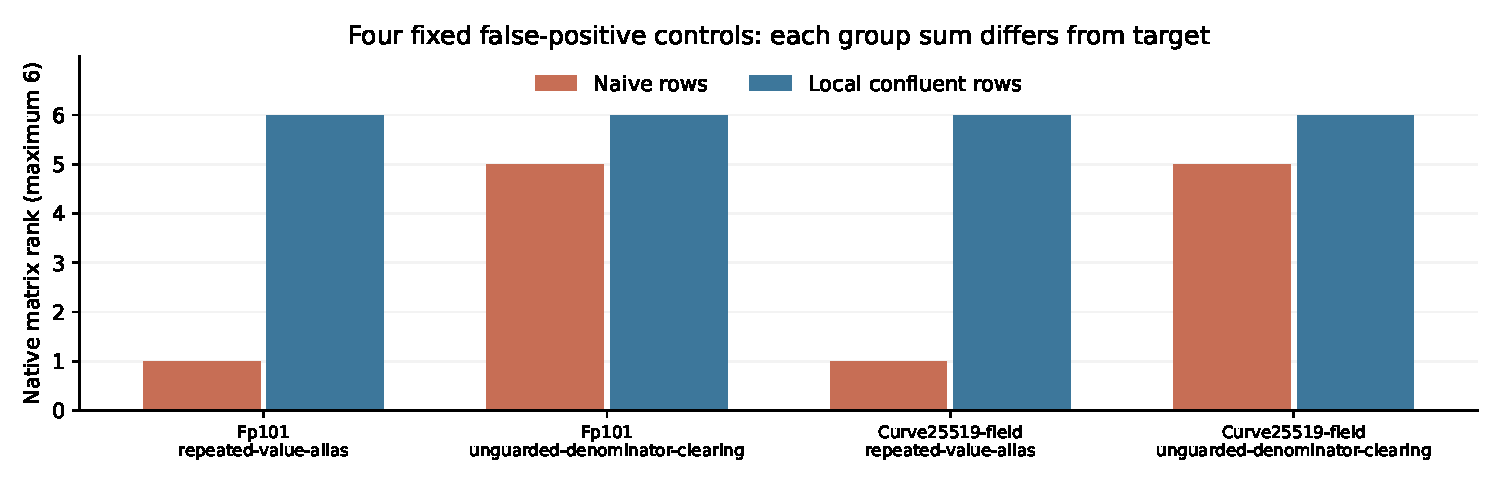
\includegraphics[width=\linewidth,height=58mm,keepaspectratio]{counterexample-ranks.pdf}
\end{center}
\small Four fixed native cases; ranks are copied directly from the retained
native output. Every group sum differs from its target. No sampling,
uncertainty interval, timing or speed interpretation.\normalsize

\newpage
{\Large Why the corrections matter}\par
\textbf{Aliases require jets.} Six distinct raw IDs carrying $G$ against $7G$
give identical ordinary value rows and a false zero determinant. The true
sum is $6G$. Confluent evaluation restores rank6. These are synthetic indexed
point controls, not an assertion of six aliases in the huge original base.

\textbf{Clearing a denominator creates false roots.} On $G,2G,\ldots,6G$
against $R=-G$, the cleared row
\[
 (x-r,\;x(x-r),\;y(x-r),\;x^2(x-r),\;xy(x-r),\;y+s)
\]
is zero at $G=-R$. Correct local sections restore rank6. At $P=R$ multiply
sections by $t=x-r$; at $P=-R$ use the removable quotient. For other points
the denominator is a unit. Hasse coefficients use only division by $2y(P)$;
the sixth-order coefficient supports multiplicity-six evaluation.

Both defects were reproduced in both fields. The toy controls use
$G=[8](2,17)$ of order13; actual controls use $G=[8](9,\sqrt{f(9)})$.
All28 multiplicity patterns over $G,2G,3G$ and two distinct-point tuples use
the protocol's fixed targets. Actual points are public mathematical controls,
not a claimed subset of the original torus factor base. All raw matrices,
points and section vectors are retained.

\textbf{The next exponent question.} In the generic chart the shared unknown
section coefficients obey
\[
 (x_i-r)(c_0+c_1x_i+c_2y_i+c_3x_i^2+c_4x_iy_i)
       +c_5(y_i+s)=0.
\]
Require a nonzero projective coefficient vector, all original guards and the
confluent/pole branches. The equations are linear in the coefficients and
cubic in coordinate features, total degree at most4 before quadratic lifting.
No replacement full-base compiler has been implemented.

For distinct geometric members, splitting rows into triples gives the standard
20-term Laplace/Pluecker pairing for the determinant \emph{value}. This is not
an existence operator: $V_{xy}=x-y$ has rank at most2, while its zero-indicator
matrix on distinct field labels is the full-rank identity. Across aliases,
global jet multiplicities also affect half representations.

Seek an implicit feature construction \emph{and} zero-extracting query with
original witnesses. Materializing $B^3$ triples already costs $N^{1/2}$ at
$B\asymp N^{1/6}$. The earlier target of more than $B$ usable tagged rows in
$B^{3-\varepsilon}$ total work retains its full setup/yield/kernel/recovery
contract. A small candidate-verification matrix alone supplies no such bound.

\textbf{Reproduction and proof scope.} Source commit
\texttt{727d40ab01bd306807836d762f4ac51ee429e37e} preceded the one final
controls call. Nine source/contract inputs, seven compiled-in hashes and a
17976-byte archive bind a separately copied953248-byte executable (SHA256
prefix\texttt{0eb6ccd2128f0780}). PRECALL was not overwritten; POSTCALL records
exit0 and unchanged source/binary. Full1736065-byte JSON is retained and
losslessly compressed to71625bytes. Unit2/fmt/strictClippy/release build pass.
These are producer records, not signed execution proof or a performance result.

The pinned Lean project checks one literal native Fp101 matrix/section.
Two named certificate endpoints and the101-primality instance pass the
focused build and maintained direct axiom audit: three declarations, zero
failing/trusted-native; only propext, Classical.choice and Quot.sound.
The full wrapper has no usable receipt during a disk-space failure and stays
unconfirmed. Generated caches were cleaned; evidence retained. No formal
geometric/native conversion is claimed. Native PCC-20261117-b77508 remains
unsigned/unverified.

\textbf{Prior art.} \href{https://arxiv.org/pdf/cs/0507026}{Cheng, section2/Theorem1};
\href{https://arxiv.org/pdf/1501.01138}{Li--Wan--Zhang, section4};
\href{https://drops.dagstuhl.de/entities/document/10.4230/LIPIcs.SoCG.2023.22}{Cardinal--Sharir};
\href{https://websites.umich.edu/asnowden/teaching/2013/679/L02.html}{Snowden, Math679}.
Variable-arity NP-hardness and real-RAM algorithms do not establish fixed-six
prime-field bounds. KB and Conductor are unavailable (127; documented fallback).
No novelty, paid run, solver campaign or scaling claim. Old frozen evidence,
criteria and canonical performance graphs remain unchanged.
\end{document}
